\section{Theorie}
\label{sec:theorie}
%
\subsection{Die Struktur von Kristallen}
%
Räumlich periodische Anordnungen von Atomen oder Molekülen werden als Kristalle bezeichnet. Sie stellen eine
in der Natur sehr häufig vorliegende Struktur von Festkörpern dar. Darstellen lassen sich Kristalle über
\textbf{Gitterstrukturen}. Die einzelnen Gitterpunkte bezeichnet man als \textbf{Basis} des Gitters. Sie bestehen
aus Atomen oder Molekülen. Die einzelnen Basen sind jeweils in bestimmten Strukturen angeordnet. Die Definition
dieser Strukturen findet dabei über drei Vektoren statt: die \textbf{fundamentalen Translationen}.\\
Sie spannen das Gitter auf, indem sie als Linearkombinationen jeden Punkt im Gitter definieren. Aufgrund ihrer
Symmetrie weisen die Gitter Translationssymmetrien auf. Sie werden also durch die von den drei fundamentalen
Translationen definierten Verschiebungen wieder in sich selbst überführt. \\
Als \textbf{Elementarzelle} wird die kleinste Einheit bezeichnet, die die Struktur eines Kristalls vollkommen
festlegt. Kristalltypen können also anhand ihrer Elementarzellen unterschieden werden. Die Darstellung eines
Kristalls durch Kombination von Elementarzellen ist allerdings nur bei einatomigen Basen möglich.\\
Prinzipiell existieren unendlich viele verschiedene Gittertypen. Die Zahl dieser Typen lässt sich jedoch über
die Betrachtung von Symmetrieeigenschaften auf die $14$ sogenannten Bravais-Gitter eingrenzen. Diese sind in
Abbildung~\ref{fig:bravais} definiert.
%
\begin{figure}[htb]
  \centering
  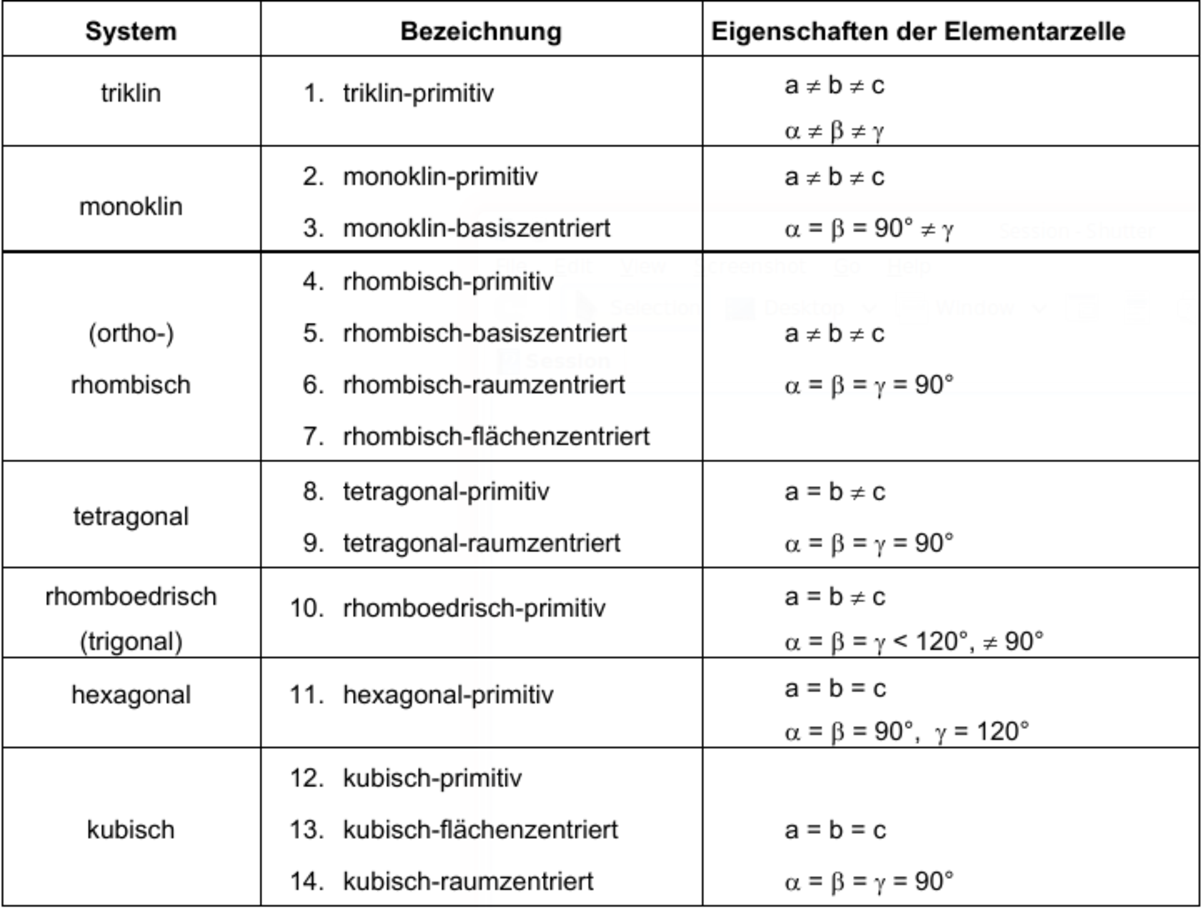
\includegraphics[width=0.8\textwidth]{figures/plot_bravais.pdf}
  \caption{Die $14$ verschiedenen Bravais-Gitter und ihre Eigenschaften \cite{V41}.}
  \label{fig:bravais}
\end{figure}
%
\subsection{Kubische Kristalle}
%
Eine Kristallstruktur, welche in der Natur häufig vorliegt, ist die kubische Kristallstruktur. Auch die im
Rahmen dieses Experimentes untersuchten Kristalle fallen in diese Kategorie. Das kubische Gitter lässt sich
in verschiedene Typen aufteilen. Das \textbf{kubisch-primitive} Gitter besitzt eine Elementarzelle, welche
ein Atom enthält. Dieses ist auf die acht Ecken des Würfels verteilt. Das \textbf{kubisch-raumzentrierte}
Gitter enthält insgesamt zwei Atome in der Elementarzelle. Es besitzt zusätzlich zum kubisch-primitiven
Gitter ein weiteres Atom in der Mitte des Würfels. Die Angabe der Postionen der Atome innerhalb der
Elementarzelle ist für die Definition der Gitter essentiell. Dazu werden die Abstände der Atome von einem
beliebig gewählten Ursprung innerhalb der Elementarzelle als Vielfache der Achsenlängen angegeben, die die
Zelle aufspannen. So befinden sich die Atome des kubisch-raumzentrierten Gitters beispielsweise an den
Punkten $\begin{pmatrix}0, & 0, & 0 \end{pmatrix}$ (Eckenatom) und $\begin{pmatrix}0.5, & 0.5, & 0.5 \end{pmatrix}$
(Mittenatom). Das \textbf{kubisch-flächenzentrierte} Gitter enthält zusätzlich zum kubisch-raumzentrierten Gitter
noch Atome auf den Seitenflächen des Würfels. So befinden sich insgesamt $4$ Atome innerhalb der Elementarzelle.
Sie besitzen die Positionen $\begin{pmatrix}0, & 0, & 0 \end{pmatrix}$, $\begin{pmatrix}0.5, & 0.5, & 0 \end{pmatrix}$,
$\begin{pmatrix}0.5, & 0, & 0.5 \end{pmatrix}$ und $\begin{pmatrix}0, & 0.5, & 0.5 \end{pmatrix}$.\\
Kristalle können auch durch Zusammensetzung von kubischen Gittern definiert werden. Einige wichtige zusammengesetzte
kubisch-flächenzentrierte Strukturen werden im Nachfolgenden beschrieben.\\
Die \textbf{Diamant-Struktur} besteht aus zwei kubisch-flächenzentrierten Gittern, die um ein Viertel der Atomdiagonalen
zueinander versetzt sind. Die Elementarzelle enthält $8$ Atome. Diese Gitterstruktur tritt beispielsweise bei
Verbindungen der vierwertigen Elemente C, Si und Ge auf.\\
Die \textbf{Zinkblenden-Struktur} entspricht der Diamant-Struktur, wobei sich die Atomsorten der ineinander gedrehten
Gitter unterscheiden. Diese Struktur lässt sich beispielsweise bei Zinksulfid finden. \\
Die \textbf{Steinsalz-Struktur} entspricht weitgehend der Zinkblenden-Struktur. Die beiden Gitter sind hierbei allerdings
statt einer viertel Raumdiagonalen eine halbe Raumdiagonale zueinender versetzt. Diese Struktur lässt sich bei NaCl
vorfinden.\\
Eine zusammengesetzte Verbindung aus kubisch-primitiven Gittern findet sich bei der sogenannten \textbf{Cäsiumchlorid-Struktur}.
Diese besteht aus zwei unterschiedlich besetzten kubisch-primitiven Gittern, die um eine halbe Raumdiagonale zueinander verschoben
sind. Daher befinden sich zwei Atome in der Elemetarzelle. \\
Schließlich existiert eine weitere Struktur aus kubischen Gittern: die \textbf{Fluorit-Struktur}. Hierbei handelt es sich um drei
kubisch-flächenzentrierte Gitter, die jeweils um $\sfrac{1}{4}$ bzw. $\sfrac{3}{4}$ der Raumdiagonalen zueinander verschoben sind.
Hier befinden sich folglich $12$ Atome in einer Elementarzelle.
%
\subsection{Abstände von Netzebenen}
%
Der Begriff \textbf{Netzebenen} bezeichnet die Ebenen innerhalb eines Kristalls, in welchen Atome des Kristalls liegen. Aufgrund
der räumlichen Periodizität des Kristalls existieren stets viele zueinander parallele Ebenen, die damit eine Ebenenschar bilden.
Die Lage dieser Ebenen lässt sich mit Hilfe der sogenannten Millerschen Indices beschreiben. Die Schnittpunkte der Ebenen mit den
Achsen eines zu den Kristallachsen parallelen Koordinatensystems werden dazu in Einheiten der fundamentalen Translationen bestimmt.
Hieraus werden die Kehrwerte gebildet und evtl. durch Multiplikation mit einer geeigneten Zahl natürlich gemacht.\\
Der Abstand dieser Netzebenen lässt sich mit Hilfe der Millerschen Indices über geometrische Überlegungen nach
%
\begin{align}
  d=&\frac{1}{\sqrt{\frac{h²}{a²}+\frac{k²}{b²}+\frac{l²}{c²}}}, \; \text{bzw} \\
  d=&\frac{a}{\sqrt{h²+k²+l²}}
  \label{eq:d}
\end{align}
%
für kubische Systeme berechnen.
%
\subsection{Beugung von Röntgenstrahlen an Kristallen}
%
Röntgenstrahlung stellt elektromagnetische Strahlung dar, die mit elektrischer Ladung in Wechselwirkung tritt. Die Wechselwrikung
von Röntgenstrahlung mit der Ladung in der Elektronenhülle und dem Atomkern eines Atoms in einem Kristall kann als klassischer
Streuprozess betrachtet werden. Durch die Beschleunigung im elektrischen Feld dieser Atome wird die Ladung zur Emmission von
elektromagnetischer Strahlung angeregt. Die strenge räumliche Periodizität innerhalb des Kristalls ist dabei Grundvorraussetzung
für das Auftreten von Interferenz bei der Röntgenstrahlung.\\
Ist dies gegeben, bilden sich je nach Gangunterschied der gestreuten Strahlung Interferenzmuster aus Verstärkung und Auslöschung aus.
Die Abhängigkeit dieser Verteilung vom Raumwinkel kann mit Hilfe eines Goniometers bestimmt werden. Hierbei werden
Fotofilme durch das Auftreffen von Röntgenstrahlung geschwärzt, sodass die Interferenzen auf eine zweidimensionale
Fläche abgebildet werden. Mit Hilfe dieses Verfahrens werden die mikroskopischen Abmessungen des Kristalls über
makroskopische Variablen messbar.\\
Das Verhalten eines mit Ladung $q$ geladenen Teilchens der Masse $m$ in einem unpolarisierten elektrischen Feld ist
das eines Herzschen Dipols. Daher gibt es eine Strahlung der Intensität
%
\begin{equation}
  I_e(r,\theta)=I_0\left(\frac{\mu_0q²}{4m\pi}\right)^2\frac{1}{r^2}\cdot\frac{1+\cos(2\theta)²}{2}
\end{equation}
%
ab. Aufgrund der im Vergleich zu den Elektronen um einige Größenordnungen größeren Masse des Atomkerns liefert die Streuung an
Elektonen den Hauptbeitrag.\\
Die Atome besitzen dabei eine ausgedehnte Elektronenhülle, an welcher die Streuung stattfindet. Wäre die Ausdehnung der
Hülle klein gegenüber der Wellenlänge der Röntgenstrahlung, so wäre die Streuintensität proportional zur Gesamtladung
und damit der Ordnungszahl der vorliegenden Elemente. Da die Wellenlänge des Röntgenlichtes allerdings in die Größenordnung
der Ausdehnung der Elektronenhülle fällt, finden Interferenzen zwischen den einzelnen Streuprozessen in der Elektronenhülle
statt. Die Streuung an den Elektronen findet aufgrund der räumlichen Ausdehnung nicht gleichzeitig statt. Dies erzeugt den
für Interferenz benötigten Phasenunterschied innerhalb der gestreuten Strahlung.\\
Die Beschaffenheit dieser Wechselwirkung wird beschrieben durch den \textbf{Atomformfaktor} $f$. Dieser ist abhängig von
der Elektronendichteverteilung $\rho(\vec{r})$. Um also $f$ zu bestimmen, ist über die gestreuten Wellen mit zugehöriger
Phase zu integrieren. Für den Phasenunterschied gilt dabei:
%
\begin{equation}
  \upD\phi=2\pi\vec{r}(\vec{k}-\vec{k}_0) \; .
\end{equation}
%
Somit ist $f$ nach
%
\begin{equation}
  f=\int_\text{Hülle}\exp(-i\upD\phi)\rho(\vec{r})\upd^3r=\int_\text{Hülle}\exp(-2i\pi\vec{r}(\vec{k}-\vec{k}_0))\rho(\vec{r})\upd^3r
\end{equation}
%
zu berechnen. Hierbei wird deutlich, dass $f$ die Fourier-Transformierte von $\rho(\vec{r})$ ist.\\
Diese Überlegungen lassen sich analog für die Interferenz der an verschiedenen Atomen in der Elementarzelle gestreuten Wellen treffen.
Für die Phasendifferenz einer Welle, die an einem im Ursprung liegenden Atom gestreut wird, zu der an einem am Ort $\vec{r}_j$
liegenden Atom gestreuten gilt:
%
\begin{equation}
  \upD\phi_j=2\pi\vec{r}_j\cdot(\vec{k}-\vec{k}_0)
\end{equation}
%
Um die Amplitude für die Streuung innerhalb der Zelle zu berechnen, muss nun unter Berücksichtigung der einzelnen Atomformfaktoren
$f_j$ für die verschiedenen Atomtypen über alle Atome in der Elementarzelle summiert werden.
%
\begin{equation}
  A=\sum_jf_j\exp(-2i\pi\vec{r}_j(\vec{k}-\vec{k}_0))I_e
\end{equation}
%
Werden die Ortsvektoren nun noch durch die Basisvektoren $\vec{a},\,\vec{b},\,\vec{c}$ der Elementarzelle dargestellt, folgt
die Strukturamplitude zu
%
\begin{equation}
  S:=\sum_jf_j\exp(-2i\pi(x_j\vec{a}+y_j\vec{b}+z_j\vec{c})(\vec{k}-\vec{k}_0))I_e \; .
  \label{eq:strukturamplitude}
\end{equation}
%
In der praktischen Durchführung ist die Richtung der ein- bzw. ausfallenden Strahlung ebenfalls zu berücksichtigen. Die Röntgenstrahlung wird aufgrund
der geringen Streuamplitude einzelner Elektronen an sehr vielen Kristallebenen gestreut. Für konstruktive Interferenz muss dabei der
entstehende Gangunterschied zwischen an verschiedenen Ebenen gestreuter Strahlung ein ganzzahliges Vielfaches der Wellenlänge betragen.
Daraus folgt über geometrische Betrachtungen eine Bedingung an den Sreuwinkel: die Braggsche Bedingung. Diese besagt, dass konstruktive
Interferenz nur stattfinden kann, wenn
%
\begin{equation}
  n\cdot\lambda=2\cdot d\cdot\sin(\theta)
  \label{eq:bragg}
\end{equation}
%
gilt.
%
\subsection{Das Debye-Scherrer Verfahren}
%
Im Rahmen des Debye-Scherrer-Verfahrens wird eine Probe mit monochromatischem Röntgenlicht bestrahlt. Die Winkel der dabei auftretenden
Bragg-Reflexe werden ausgemessen. Ziel ist dabei das Finden der zugehörigen Netzebenen bzw. das Ausmessen der ausbleibenden Reflexe. Nach
Gleichung~\eqref{eq:strukturamplitude} existieren Netzebenen, die aufgrund ihrer Millerschen Indices eine Streuamplitude besitzen, die
stets Null ist. Hier lässt sich also auch das Ausbleiben bestimmter Reflexe überprüfen. Im Allgemeinen treten bei Bestrahlung mit
Röntgenlicht keine Bragg-Reflexe auf, da bei einem Kristall zufällig exakt der Bragg-Winkel für eine beobachtbare Interferenz getroffen
werden müsste. Daher wird eine fein pulverisierte, kristalline Probe in zylindrischer Form verwendet. Da hier die Orientierungen der
Kristalle statistisch über alle Raumwinkel verteilt sind, treten stets einige Reflexe auf. Um dabei etwaige Grobkörnigkeiten des
Probenmaterials zu kompensieren, wird die Probe während der Messug permanent gedreht, und so von allen Seiten nacheinender bestrahlt.\\
Bei dem Versuchsaufbau treten einige systematische Fehler auf, die einer Korrektur bedürfen. Die Probe absorbiert die auf sie treffende
Röntgenstrahlung fast gänzlich. Beugung findet daher nur auf dem aüßeren Rand des Probenzylinders statt. Aufgrund der Ausdehnung des
Zylinders wird daher tendenziell ein zu großer Öffnungswinkel der Strahlung gemessen. Deshalb wird der Korrekturfaktor
%
\begin{equation}
 \frac{\upD a_A}{a}=\frac{\rho}{2R}\left(1-\frac{R}{F}\right)\frac{\cos(\theta)²}{\theta}
\end{equation}
%
für die bestimmte Gitterkonstante $a$ verwendet. Hierbei ist $\rho$ der Probenradius, $R$ der Kameraradius ($\SI{57,3}{\milli\meter}$)
und $F$ der Abstand der Probe vom Fokus der Kamera ($\SI{130}{\milli\meter}$).\\
Des Weiteren kann auch nicht gewährleistet werden, dass die Probenachse exakt mit der Achse des Filmzylinders zusammenfällt. Daher
findet in der gebeugten Strahlung auf allen Seiten des Zylinders eine Verschiebung gegen die wahre Richtung statt. Um diesen
Umstand zu berücksichtigen, wird die Korrektur $\upD a_V$ bei der Bestimmung der Gitterkonstanten berücksichtigt:
%
\begin{equation}
  \frac{\upD a_V}{a}=\frac{V}{R}\cos(\theta)² \; .
\end{equation}
%
Diese Korrektur übernimmt dabei bei größeren Winkeln die entscheidende Rolle, während $\upD a_A$ im Kleinwinkelbereich dominiert.
Zwischen den Korrekturen gilt näherungsweise die Relation
%
\begin{equation}
  \upD a_\text{ges}=\upD a_V+\upD a_A\propto\cos{\theta}² \; .
\end{equation}
%
Lineare Ausgleichsrechnung für die berechnete Gitterkonstante $a$ in Abhängigkeit von $\cos{\theta}²$ ergibt damit über den
$y$-Achsenabschnitt den besten Wert für $a$.
